\documentclass[11pt,a4paper]{article}
\usepackage[T1]{fontenc}
\usepackage[utf8]{inputenc}
\usepackage{lmodern,microtype,amsmath,amssymb,amsthm,booktabs,longtable,graphicx}
\usepackage[margin=23mm]{geometry}
\usepackage[hidelinks]{hyperref}
\usepackage{fancyhdr}
\pagestyle{fancy}\fancyhf{}\fancyhead[L]{FIN: thirty adaptive falsification studies}
\fancyhead[R]{ST8549--ST8578}\fancyfoot[C]{\thepage}
\setlength{\headheight}{14pt}\setlength{\emergencystretch}{3em}
\newtheorem{theorem}{Theorem}
\newtheorem{proposition}[theorem]{Proposition}
\newtheorem{corollary}[theorem]{Corollary}
\newcommand{\one}{\mathbf 1}
\newcommand{\diag}{\operatorname{diag}}
\newcommand{\Tr}{\operatorname{Tr}}
\newcommand{\TV}{\operatorname{TV}}
\newcommand{\E}{\mathbb E}
\newcommand{\Prob}{\mathbb P}
\hypersetup{pdftitle={What FIN Determines and What It Does Not: Thirty Adaptive Falsification Studies},pdfauthor={Krzysztof Żuchowski}}
\begin{document}\hypersetup{pageanchor=false}
\begin{titlepage}\centering\vspace*{18mm}
{\Huge\bfseries What FIN Determines\par}
\vspace{3mm}{\Huge\bfseries and What It Does Not\par}
\vspace{10mm}{\LARGE Thirty Adaptive Falsification Studies\par}
\vspace{5mm}{\Large Signed kernels, dual dynamics, collective information,\par}
{\Large and a conditional operational bridge\par}
\vspace{12mm}{\Large Programmes ST8549--ST8578\par}
\vspace{10mm}{\Large Krzysztof \.Zuchowski\par}
\vspace{3mm}{Independent Researcher --- Fractal Information Theory Project\par}
{ORCID: 0009-0002-0909-3613\par}
\vspace{9mm}{6 September 2026\par}
\vfill
\begin{minipage}{.89\textwidth}
One analytical and computational campaign, organized into thirty bounded
investigations. Every step states its premises, an explicit result and the
reason for the next step. The central result is a conditional uniqueness
and stability theorem for collective Markov dynamics, together with an
explicit family proving that the presently supplied FIN data do not enforce
its decisive premise.
\end{minipage}
\vfill{\small English research preprint. CC BY 4.0. AI-assisted research; no external audit.}
\end{titlepage}\hypersetup{pageanchor=true}

\begin{abstract}
The strict finite FIN kernel supports exact spectral calculus, but that
calculus does not identify a unique microscopic or physical realization.
We test this statement constructively rather than treating it as a universal
philosophical prohibition. A positive double cover retains the signs of the
canonical legacy profile; its coarse generator is nevertheless not strict.
Repeated measurements of the strict Hamiltonian produce squared edge rates,
whereas an exact Lindblad heat embedding leaves independent coherence data.

The principal counterexample is a family of collective Markov generators
with the same strict singleton dynamics, every singleton path law, product
equilibrium, detailed balance, exchangeability, projective consistency and
graph symmetries. Their pair records differ. Neither entropy nor consistency
alone selects independence. Conversely, autonomous singleton generators and
zero simultaneous-pair activity force the independent tensor-sum generator.
A nonnegative pair-activity budget also bounds the error in the full
finite-time transition law. This supplies an explicit, falsifiable extra
premise, not a derivation of that premise from FIN.

Finite resolution, loss and unknown detector calibration are then used to
attack the proposed test. A conditional finite-shot protocol survives known
resolution-preserving loss; uncalibrated merging can make distinct models
exactly indistinguishable. Additional counterexamples show that a static
propagator does not determine nonlinear interactions or hidden memory.
No physical units, laboratory observations, selector closure, legacy role
transfer, Standard Model or gravitational dynamics are obtained.
\end{abstract}

\tableofcontents\newpage

\section{Executive result and epistemic scope}

The strongest conclusion of this campaign is not that FIN is impossible,
and not that it has become a Theory of Everything. It is the following
sharpened statement:
\begin{quote}
Within a precisely declared finite Markov realization class, the present
FIN data leave a genuine collective-dynamics ambiguity. A nonnegative,
conditionally observable pair-coincidence budget isolates one missing
composition premise. Setting that budget to zero yields a unique generator;
bounding it yields a quantitative approximation theorem. FIN has not yet
supplied the law that sets or bounds it.
\end{quote}

This is useful because an unspecified ``missing physical principle'' becomes
a concrete mathematical question. It is only one part of the physics bridge:
composition locality is not spatial locality, no-signalling, a light cone,
an action unit, a quantum measurement postulate or an actual detector.

We use the categories \emph{Proven}, \emph{Strong evidence},
\emph{Moderate evidence}, \emph{Speculative} and \emph{Refuted}.
Here, Proven always means that the displayed mathematical statement follows
from its displayed premises by the accompanying proof. Numerical residuals,
spectral values and power calculations are floating checks unless explicitly
identified as exact rational or symbolic tests. Refuted refers to a stated
implication, not to the entire FIN programme. No mathematical priority or
independent peer review is asserted.

\subsection{Repository coverage and limitations}

The initial inventory covered the repository file list and the complete
AGENTS section index. The selected reading included the top-level guardrails,
current ST8547/ST8548 frontier, relevant earlier kernel, duality, refinement,
configuration and source-obstruction sections, SUMMARY\_GROK.md and the
current theory compendium. The latest committed head at the start was
\texttt{295cc900}; the then-visible scientific inventory, excluding the named
third-party directories, contained about 33,000 files. Existing local changes
were preserved. No remote pull or heavy algebra campaign was started.

This is \emph{not} a fresh line-by-line verification of every historical file
or every assertion in the approximately one-megabyte AGENTS chronology.
Historical results were used as a state map; the claims promoted in this
report have their own proofs or counterexamples below. In particular, earlier
empty generated status payloads and hash matches are not counted as research
evidence. Thirty steps here means thirty bounded investigations, not thirty
independent papers or thirty universal new theorems.

The campaign proceeded through six checkpoints: signs and vertex dynamics
(1--5), measurement constructions (6--10), microscopic consistency (11--15),
pair locality and false count tests (16--20), operational identifiability
(21--25), and independent action/memory counterexamples plus synthesis
(26--30). The results and next-step rationales are retained in
\texttt{results.json}; the appendix gives the full chain. Replay is
deterministic and is not itself a new adaptive discovery run.

\section{Founding interpretation and the mathematical inputs}

FIN originates in the hypothesis that the nadsoliton itself is primordial,
self-coupled fractal information in a persistent solitonic state, with the
intended order nadsoliton $\to$ light $\to$ matter $\to$ emergent observer.
No separate information substrate is inserted beneath that object. This
ontology is the motivation, not an experimentally established conclusion.
Likewise, persistent modes, self-learning, maximum resonance, octave labels
and fractal compression do not by themselves define a nonlinear soliton
equation, physical matter, a metric or a calibrated clock.

\subsection{Strict and legacy must remain different typed objects}

Let $d(i,j)=\min(|i-j|,12-|i-j|)$ and set diagonal weights to zero. The
supplied strict profile and the canonical legacy instance used here are
\begin{align}
 W_{ij}&=\frac{\cos(0.18575d+0.16250)}{1+d^{9/5}},\\
 V_{ij}&=4\log2\,\frac{\cos(\pi d/4+\pi/6)}{1+0.01d}.
\end{align}
The latter is also one member of the reconstructed Legacy* class with free
amplitude and damping. Statements about this frozen member must not be
promoted to every historical legacy variant. The strict phase decimals are
supplied frozen parameters, not newly derived constants.

For strict, every angle on $d=1,\ldots,6$ lies strictly between zero and
$\pi/2$. Thus $W_{ij}>0$ off the diagonal. With
\[
 A=\diag(W\one)-W=sI-W,\qquad
 s\simeq1.6603072787660986,
\]
the exact identity
\[
 f^*Af=\frac12\sum_{i,j}W_{ij}|f_i-f_j|^2\geq0
\]
proves positivity. We use row generators $Q=-A$ for stochastic matrices and
column probability vectors $\dot p=Q^Tp=-Ap$; symmetry makes the matrices
coincide, not the conventions.

The finite spectral theorem gives
\[
 U_t=e^{-itA},\qquad P_t=e^{-tA},\qquad
 G_z=(A+zI)^{-1},\qquad C_t=\cos(t\sqrt A).
\]
These share spectral projectors. They are respectively a unitary group,
Markov heat semigroup, resolvent, and second-order wave evolution factor.
$U_t$ has frequencies $\lambda$, whereas $C_t$ has $\sqrt\lambda$.
They do not supply the same operational law, and no SI units are assigned.

\section{Signed legacy: a constructive dilation and its obstruction}
\label{sec:signed}

\begin{theorem}[Positive double cover; rounds 1--4]
For any real symmetric zero-diagonal $V$, put
$V_+=\max(V,0)$, $V_-=\max(-V,0)$ entrywise. Define
\[
 \widetilde W=\begin{pmatrix}V_+&V_-\\V_-&V_+\end{pmatrix},\quad
 \widetilde L=\diag(\widetilde W\one)-\widetilde W,
 \quad E_\pm=\frac1{\sqrt2}\binom{I}{\pm I}.
\]
Then
\begin{align}
 \widetilde L E_+&=E_+L_{|V|},&
 L_{|V|}&=\diag(|V|\one)-|V|,\\
 \widetilde L E_-&=E_-L_V^{\rm sign},&
 L_V^{\rm sign}&=\diag(|V|\one)-V\succeq0.
\end{align}
Mass collapse $C=(I\ I)$ obeys $C\widetilde L=L_{|V|}C$.
\end{theorem}
\begin{proof}
Block multiplication gives the intertwining identities. Positivity also
follows directly from
$f^*L_V^{\rm sign}f=\sum_{i<j}|V_{ij}|\,
|f_i-\operatorname{sgn}(V_{ij})f_j|^2$.
The collapse identity has no dependence on the edge signs. Exponentiating
the finite identities gives the corresponding semigroup relations.
\end{proof}

The odd coordinate is a \emph{difference} between sheet populations, not a
probability vector. It retains a signed amplitude without interpreting
negative numbers as rates. This is standard signed-graph structure
\cite{zaslavsky}, applied explicitly here; it is not a new strict kernel.

The raw legacy Laplacian $L_V^{\rm raw}=\diag(V\one)-V$ satisfies
\[
 L_V^{\rm sign}=L_V^{\rm raw}+2\diag(V_-\one).
\]
For this circulant instance the shift is a scalar
$c\simeq27.8057289704$. Therefore
\[
 e^{-itL_V^{\rm sign}}=e^{-ict}e^{-itL_V^{\rm raw}},\qquad
 e^{-tL_V^{\rm sign}}=e^{-ct}e^{-tL_V^{\rm raw}}.
\]
The first factor is a global unitary phase; the second is a real attenuation.
Removing it is not a probability-preserving gauge change. This is another
reason to keep the operational meanings of the dual channels distinct.

\begin{proposition}[Frustration obstruction]
The canonical legacy instance cannot be switched to all-positive weights
by vertex signs, nor made into positive rates by a positive diagonal
similarity transformation.
\end{proposition}
\begin{proof}
In triangle $(0,1,2)$ the two length-one edges are positive and the
length-two edge is negative: $\cos(5\pi/12)>0$ and
$\cos(2\pi/3)<0$. The product of edge signs around a cycle is unchanged
under $V_{ij}\mapsto\sigma_iV_{ij}\sigma_j$. An all-positive triangle
would have positive product. A positive similarity multiplies each edge by
a positive ratio and cannot change any sign in the first place.
\end{proof}

The computed legacy signed-sector lowest eigenvalue is about $6.42867$;
the raw Laplacian has a negative eigenvalue about $-21.3771$.
These numbers are checks, while the sign obstruction is analytic.
There are 112 negative-product triangles in the finite enumeration.
The cover forgets all signs under mass collapse and produces $|V|$, not
$W$. Even the best scalar multiple of $|V|$ has relative Frobenius error
about $0.8834$ against strict. Exact nonproportionality already follows
from unequal ratios at two distances. No amplitude fit is used as a source.

This construction does not complete legacy into strict, select a physical
sign, explain electroweak or gravitational roles, or supply a fractal
$12\to24$ refinement law. Its extra sheet is a mathematical sign carrier.

\section{Dual dynamics survives; a unique operational identification does not}
\label{sec:quantum}

\subsection{Short-time falsification and repeated measurements: rounds 5--7}

For $i\ne j$, Taylor expansion gives
\[
 (P_t)_{ij}=tW_{ij}+O(t^2),\qquad
 |(e^{-itH})_{ij}|^2=t^2|H_{ij}|^2+O(t^3).
\]
For nonzero $W$ no positive linear time calibration identifies these
transition records near zero. This does not refute common spectral calculus;
it refutes equality of these specified vertex-record laws.

\begin{proposition}[Measured small-step limit]
If each step of duration $\delta$ applies $e^{-i\sqrt\delta H}$ followed
by a complete vertex measurement, its stochastic matrix $S_\delta$ obeys
\[
 S_\delta=I+\delta Q_H+O(\delta^{3/2}),\qquad
 (Q_H)_{ij}=|H_{ij}|^2\quad(i\ne j).
\]
For fixed $T$, $S_{T/n}^{\,n}\to e^{TQ_H}$. Without the
$\delta^{-1/2}$ Hamiltonian scaling, the same frequent-measurement limit
freezes the vertex transitions.
\end{proposition}
\begin{proof}
Expand the unitary to second order in $\sqrt\delta$. Off-diagonal
probabilities are $\delta|H_{ij}|^2+O(\delta^{3/2})$; stochasticity fixes
the diagonal. The finite matrix product limit follows from the logarithm
near the identity, or a telescoping estimate with error $O(n^{-1/2})$.
With an unscaled Hamiltonian the off-diagonal step probability is
$O(\delta^2)$ and $n\delta^2\to0$.
\end{proof}

For $H=A$ the limiting rates are $W_{ij}^2$. Since the six strict weights
differ, no common clock makes those rates equal to $W_{ij}$. One can
\emph{compile} the desired limit by choosing
\[
 H_{ij}=\sqrt{W_{ij}}e^{i\theta_{ij}},\quad
 \theta_{ji}=-\theta_{ij},\qquad H_{ii}\in\mathbb R.
\]
This is a construction with new phase and diagonal data. It is not
$H=A$. Changing one real edge sign preserves all compiled rates but changes
a triangle phase and $\Tr(H^3)$; hence even its coherent spectrum need not
be preserved. Gauge-invariant loop phases survive diagonal rephasing.

\subsection{Exact quantum heat embedding and a coherence ambiguity: rounds 8--10}

Use the rank-one jumps $L_{ji}=\sqrt{W_{ij}}|j\rangle\langle i|$ and set
\begin{align}
 \mathcal D_W(\rho)&=\sum_{i\ne j}\left[
 L_{ji}\rho L_{ji}^*-	frac12\{L_{ji}^*L_{ji},\rho\}\right],\\
 \mathcal D_W(\rho)_{ii}&=(Q^Tp)_i,\quad p_i=\rho_{ii},\\
 \mathcal D_W(\rho)_{ij}&=-\tfrac12(r_i+r_j)\rho_{ij}\quad(i\ne j),
 \qquad r_i=\sum_jW_{ij}.
\end{align}
The displayed Lindblad form proves complete positivity and trace
preservation of its finite-dimensional semigroup \cite{lindblad}.
The component identities follow by direct multiplication and hold for
\emph{every} density matrix, including coherent states. Thus exact heat
populations admit a quantum extension. This is within the established
quantum-stochastic-walk framework \cite{qsw}.

For every $\gamma\ge0$ the additional vertex-dephasing generator
\[
 \gamma\left(\sum_i|i\rangle\langle i|\rho|i\rangle\langle i|-\rho\right)
\]
changes off-diagonal decay but none of those population trajectories.
Complete population records do not identify $\gamma$.

\begin{proposition}[Restricted Hamiltonian obstruction]
In the class consisting of these rank-one jumps, arbitrary vertex
dephasing and a Hamiltonian commutator, autonomous populations
$\dot p=Q^Tp$ for every density matrix require the Hamiltonian to be
diagonal in the vertex basis.
\end{proposition}
\begin{proof}
The jump and dephasing terms already give the required diagonal. The
remaining condition is
$\diag[-i(H\rho-\rho H)]=0$ for every density matrix. For each edge,
vary the phase of a small coherence in a positive two-dimensional block.
Its contribution is proportional to the imaginary part of
$H_{ij}\rho_{ji}$. Vanishing for every phase forces $H_{ij}=0$.
Conversely a diagonal Hamiltonian contributes no diagonal commutator.
\end{proof}

This excludes adding the non-diagonal strict $H=A$ in this particular
embedding while retaining exact heat for all states. It is not a theorem
about every conceivable Lindblad representation, dilation, feedback
instrument or restricted preparation class.

\subsection{Imaginary-time filtering: round 11}

For a positive contraction $P=e^{-tA}$ the operation $\rho\mapsto P\rho P$
is completely positive but generally trace decreasing. Its normalized
conditional state is
\[
 \rho\longmapsto \frac{P\rho P}{\Tr(P\rho P)}.
\]
If $P$ has two unequal eigenvalues, mixing the corresponding pure states
before filtering changes their relative weights, while filtering each pure
state first leaves it unchanged. Thus the normalized map is not affine and
cannot be a deterministic quantum channel on every input. A successful
postselection event and its probability must be retained. The analytic
identity $P_t=U_{-it}$ has not produced a Born rule or a measurement record.

\section{The central counterexample: collective dynamics hidden from all singleton laws}
\label{sec:collective}

Let $X=\{0,\ldots,11\}$ and declare a finite population state space $X^N$.
This is a mathematical completion, not a derivation of physical particles
or of the earlier $4096$-state binary configuration model. For
$x=(x_1,\ldots,x_N)$ define
\begin{align}
 (G_N^{\rm ind}f)(x)&=\sum_{k=1}^N\sum_{j\ne x_k}W_{x_kj}
       [f(x^{k\to j})-f(x)],\\
 (G_N^{\rm com}f)(x)&=\sum_{i<j}W_{ij}[f(\sigma_{ij}x)-f(x)],\\
 G_N^{(\theta)}&=(1-\theta)G_N^{\rm ind}+\theta G_N^{\rm com},
 \qquad 0\le\theta<1,
\end{align}
where $\sigma_{ij}$ exchanges vertex labels $i,j$ in \emph{every}
coordinate at once. Terms that do not change $x$ are zero.

\begin{theorem}[Explicit collective nonidentifiability; rounds 12--14 and 29]
Every member of this family has the same autonomous singleton generator
$Q=-A$ and hence every singleton path law for any supplied singleton
initial distribution. The family is exchangeable under particle-label
permutations and projectively consistent under deletion of coordinates.
Each finite $N$ member is irreducible and reversible with respect to the
same product-uniform measure. It respects every vertex symmetry of $W$.
For $N\ge2$, different $\theta$ nevertheless give different collective
transition laws.
\end{theorem}
\begin{proof}
For $f(x)=h(x_k)$, the only common transpositions that affect $f$ exchange
$x_k$ with some $j$, giving precisely
$\sum_jW_{x_kj}[h(j)-h(x_k)]$. The independent generator gives the same
result. The calculation extends to any subset of coordinates: jumps on
deleted independent coordinates vanish, and the common transpositions
restrict to the same common-transposition generator on the retained ones.
This proves strong projective consistency and singleton path equality.

Coordinate permutations commute with both constructions. Vertex symmetries
permute transpositions and preserve their weights. Each common map is an
involution with the same forward and reverse coefficient; the independent
weights are symmetric as well. Their generator matrices are symmetric, so
the uniform measure on $X^N$ is reversible. For $\theta<1$, the positive
independent part connects every configuration by single-coordinate changes,
proving irreducibility and uniqueness of this stationary distribution.

At $N=2$, the rate from $(i,i)$ to $(j,j)$ is $\theta W_{ij}$.
It is zero for the independent generator and positive for $\theta>0$.
For different parameters these entries differ. Therefore the pair
semigroups, and consequently the collective path laws, differ.
\end{proof}

The construction is compatible with the general literature on exchangeable
Markov processes, where exchangeability permits shared randomness rather
than forcing unconditional independence \cite{crane}. The proof above is
finite and does not require the general representation theorem.

All members have the same stationary occupancy multinomial distribution
and the same static Shannon large-deviation expression. Thus even the full
product equilibrium law, rather than only its entropy, fails to identify
the kinetics. If initialized in that equilibrium, the coordinates are
independent at each \emph{single instant}; their path histories need not be
independent. This distinction prevents an erroneous inference from static
factorization to dynamical tensorization.

For strict $W$, preparation $(0,0)$ and time $t=0.02$, direct exponentiation
gives
\[
 \Prob_{\theta=0}((1,1))\simeq0.0000834915,\qquad
 \Prob_{\theta=0.35}((1,1))\simeq0.0031556561.
\]
The numerical values are illustrations. The exact differing first-order
rates already prove distinguishability. No laboratory observation was made.

\section{A positive theorem: composition locality, its witness and its stability}
\label{sec:budget}

Consider \emph{any} finite continuous-time Markov generator $G$ on $X^N$,
with off-diagonal rates $g(x,y)\ge0$. The pointwise autonomous-singleton
condition is
\begin{equation}\label{eq:marginal}
 \sum_{y:y_k=j}g(x,y)=Q_{x_kj}\quad
 (j\ne x_k),\quad\text{for every }x,k,j.
\end{equation}
This is stronger than matching a mean at equilibrium or along one chosen
trajectory. Define the number of changed coordinates in one event and its
pair-activity budget by
\[
 K(x,y)=\#\{k:x_k\ne y_k\},\qquad
 B(x)=\sum_{y\ne x}g(x,y)\binom{K(x,y)}2.
\]

\begin{theorem}[Conditional uniqueness; rounds 15--16]
Under \eqref{eq:marginal}, $B(x)=0$ for every configuration if and only if
$G=\sum_k Q^{(k)}$, the independent transition generator.
No exchangeability premise is required.
\end{theorem}
\begin{proof}
All summands in $B$ are nonnegative, so $B=0$ excludes every event changing
two or more coordinates. For a fixed $x,k,j$, exactly one possible remaining
destination changes only coordinate $k$ to $j$. Equation \eqref{eq:marginal}
therefore forces its rate to be $Q_{x_kj}$. The diagonals are fixed by row
sums, proving the claimed generator. Conversely this generator changes one
coordinate per event, hence has zero budget.
\end{proof}

For a fixed initial configuration $x$, define
$f_k^x(z)=\mathbf1_{z_k\ne x_k}$. Then
\[
 \Gamma_G(f_k^x,f_l^x)(x)
 :=G(f_k^xf_l^x)(x)-f_k^x(x)Gf_l^x(x)-f_l^x(x)Gf_k^x(x)
 =\sum_y g(x,y)\mathbf1_{y_k\ne x_k,y_l\ne x_l}.
\]
Summing over $k<l$ gives $B(x)$. This uses gross changes in an event, not
cancellations of signed displacements. Merely finding zero \emph{stationary
average} cross covariance for one pair of fixed observables is insufficient:
in the common-flip counterexample such an average can vanish while $B>0$.
That false shortcut is explicitly rejected by a regression test.

\begin{theorem}[Finite-time robustness; round 17]
Under \eqref{eq:marginal}, if $\sup_xB(x)\le\varepsilon$, then for every
initial configuration and $t\ge0$,
\[
 \TV\big(e^{tG}(x,\cdot),e^{tG^{\rm ind}}(x,\cdot)\big)
 \le\min(1,2\varepsilon t).
\]
The same bound holds after mixing initial configurations with any common
initial distribution and after any common stochastic observation map.
\end{theorem}
\begin{proof}
In one row, a joint event $x\to y$ with rate $c$ and $k=K(x,y)\ge2$
replaces $k$ separate single-coordinate events of rate $c$ each, by the
singleton constraints. Its contribution to $G-G^{\rm ind}$ is
\[
 c\left[\delta_y-\sum_{l\text{ changed}}\delta_{x^{l\to y_l}}
                       +(k-1)\delta_x\right].
\]
Its row $\ell^1$ norm is at most $2kc$. Consequently
\[
 \tfrac12\sup_x\sum_y|G-G^{\rm ind}|(x,y)
 \le\sup_x\sum_{y:K\ge2}K g(x,y)
 \le2\sup_x B(x),
\]
because $k\le2\binom{k}{2}$. Apply the finite matrix Duhamel identity
\[
 e^{tG}-e^{tG^{\rm ind}}
 =\int_0^t e^{sG}(G-G^{\rm ind})e^{(t-s)G^{\rm ind}}\,ds.
\]
Stochastic multiplication contracts the relevant row total-variation norm.
Integration gives $2\varepsilon t$; total variation is at most one.
Mixtures and observation channels also contract total variation.
\end{proof}

This bounds \emph{transition distributions}, not the total variation of
entire continuous-time path records. Pathwise coupling bounds require their
own accounting. The stated bound is conservative, not claimed sharp. The
three-coordinate test has actual transition TV about $0.04513$, below its
$0.672$ bound; twelve further perturbed three-state tests passed.

\subsection{Premise removal and the meaning of independence}

Removing zero pair activity restores the common-transposition family.
Removing the singleton-rate condition permits, for example,
$2\sum_kQ^{(k)}$ with the same zero budget. Thus the two conditions are
independently needed for this characterization relative to the declared
finite Markov state space. A non-Markov model, unidentified population or
different state space is outside the theorem, not silently covered.

A product transition semigroup also does not force a product \emph{initial}
law. Initially correlated particles remain correlated at finite times.
The model specification must supply that law separately. The theorem
selects a generator, not the origin of particles, their preparation, a
physical clock or an apparatus.

\subsection{A deterministic macroscopic limit is too weak: round 18}

For each $N$, select unordered pairs of particle labels. For every vertex
transposition $(i,j)$, let it act on each selected pair at rate
$\theta W_{ij}/(N-1)$, together with independent jumps at rate
$(1-\theta)W_{ij}$ per coordinate. Each coordinate participates in $N-1$
pairs and still has precisely the generator $Q$. The family is exchangeable,
but it is not projectively consistent across $N$: deleting a partner
changes some paired events into singleton events.

In the two-state case, with all particles initially at one vertex and flip
rate $w$, the total numbers of changed coordinates have initial rates
\[
 r_1=(1-\theta)Nw,\quad r_2=\theta Nw/2,
 \qquad \mu/N=w,\quad v/N=(1+\theta)w.
\]
The empirical fraction has jumps of size at most $2/N$, total event rate
$O(N)$, and hence martingale quadratic variation $O(1/N)$ on bounded time
intervals. Its drift is the exact linear heat drift. With deterministic or
appropriately concentrated initial data, the usual elementary martingale
estimate and variation of constants yield a deterministic mean-field limit.
Nevertheless the local noise coefficient differs. We do not claim a full
central-limit theorem here. Exact projectivity, a deterministic limit and
absence of common jumps are different assumptions.

\section{From a mathematical witness to a falsifiable counting protocol}
\label{sec:detector}

\subsection{Local integer constraints, and a false finite-bin application}

For an integer-mark event process with instantaneous nonnegative rates
$c_k$, its local counting Hamiltonian is
$h(s)=\sum_kc_k(e^{ks}-1)$. Assuming the displayed moments are finite,
\[
 \kappa_2=\sum_k k^2c_k\ge|\sum_k kc_k|=|\kappa_1|,\qquad
 \kappa_4-\kappa_2=\sum_k k^2(k^2-1)c_k\ge0.
\]
Equality in the second inequality forces all nonzero marks to have
$|k|=1$. These statements concern instantaneous raw count rates, not the
finite-window cumulants of an arbitrary correlated record.

For the ST8548 strict edge test, the quadratic logarithmic-mean noise
prescription has $v/|\mu|=2/\log12<1$. This refutes its exact
interpretation as such an integer-count generator. It does not refute a
continuous Gaussian approximation or the valid Onsager gradient identity.
The nonquadratic microscopic fluctuation construction is established
literature \cite{mpr}; its FIN application is not a new universal theory.

Round 20 deliberately breaks an attempted experimental shortcut. Poisson
arrivals with rate $\lambda$, reported as at most one click in a bin of
width $\Delta$, produce a Bernoulli variable with
\[
 q=1-e^{-\lambda\Delta},\qquad
 \frac{\operatorname{Var}(\mathrm{click})}{\E(\mathrm{click})}
 =e^{-\lambda\Delta}<1.
\]
Valid microscopic jumps can therefore yield a sub-unit ratio after ordinary
thresholding. That observed ratio alone is not a falsification of Markov
microscopy or evidence for a novel FIN noise law.

\subsection{Loss that preserves resolution: round 21}

If each changed coordinate in an event is independently registered with
efficiency $0<\eta\le1$, and the instrument retains the number of changes,
then $M\mid K\sim\operatorname{Bin}(K,\eta)$. Counting pairs gives exactly
\[
 \E\binom M2=\eta^2\binom K2,
 \qquad B_{\rm observed}(x)=\eta^2 B(x).
\]
Thus the ideal zero set survives positive independent loss. An upper bound
on $B$ needs a known lower bound on efficiency. Correlated losses, unknown
merging, afterpulses, backgrounds or unobserved detector recovery states are
not licensed by this identity. It is an event-level identity, not an
uncorrected finite-bin factorial-moment formula.

\subsection{A finite-resolution null bound: rounds 22--23}

Suppose the finite Markov chain has an escape-rate bound $\Lambda$. Under
the no-joint-change null, at least two detected coordinate changes require
at least two true events. Uniformization therefore gives
\begin{equation}\label{eq:null}
 \Prob(C_\Delta\ge2)\le\Prob(\operatorname{Pois}(\Lambda\Delta)\ge2)
 \le\frac{(\Lambda\Delta)^2}{2}=:q_0.
\end{equation}
The last bound follows from
$\mathbf1_{M\ge2}\le M(M-1)/2$ and the Poisson factorial moment.
For the strict $N$-particle autonomous-marginal class, $\Lambda=Ns$ is
valid: every genuine event changes at least one coordinate and the sum of
coordinate change rates is $Ns$.

If a prepared configuration $x$ instead has joint-event detected rate
\[
 r_{\ge2}^{\rm det}(x)=\sum_y g(x,y)
     \Prob(\operatorname{Bin}(K(x,y),\eta)\ge2),
\]
the probability of exactly one uniformization proposal, realizing that
event with no others, gives the lower bound
\[
 \Prob_x(C_\Delta\ge2)\ge
 e^{-\Lambda\Delta}\Delta r_{\ge2}^{\rm det}(x).
\]
The null is $O(\Delta^2)$; a resolved common-event alternative is
$O(\Delta)$. Neither result requires approximating a finite closed-chain
count by independent Poisson edge counts.

For a completely explicit design example, take two binary coordinates,
flip rate $w=0.7$, common-flip fraction $\theta=0.2$, efficiency $\eta=0.6$
and $\Delta=0.01$. The independent and common Poisson clocks have
configuration-independent rates in this example. After thinning, the
observed count law has marks one and two with rates
\[
 c_1=2w\eta(1-\theta\eta),\qquad c_2=\theta w\eta^2,
 \qquad h(s)=c_1(e^s-1)+c_2(e^{2s}-1).
\]
Hence
\[
 q_1=1-e^{-(c_1+c_2)\Delta}(1+c_1\Delta)
 \simeq0.00053104588,
 \qquad q_0\le0.000098.
\]
With 200,000 independently reset trials, the recommended conservative rule
rejects when at least 40 bins have two or more detected changes. This rule
admits error bounds without relying on a floating binomial tail.
Under the null, for the count $Z$ of qualifying bins,
\[
 \Prob(Z\ge40)\le 2^{-40}(1+q_0)^M
 \le 2^{-40}e^{19.6}
 < (11/16)^{20}<10^{-3},
\]
using $e<11/4$. Under the supplied alternative,
$q_1\ge(1-0.014)\,0.01\,0.2\,0.7\,0.6^2=0.000496944$,
so $Mq_1/2>49$. Using $e>8/3$ gives
\[
 \Prob(Z\le39)\le2^{39}(1-q_1/2)^M
 \le2^{39}e^{-Mq_1/2}<\frac{3^{49}}{2^{108}}<10^{-9}.
\]
The simple inequalities for $e$ follow from its convergent positive Taylor
series and a geometric tail bound. The final bounds are exact rationals,
checked with integer arithmetic. Floating binomial tails supply an additional
check; their less conservative threshold 36 is not needed for the certified
rule. These are conditional design calculations, not completed experiments,
detector specifications or evidence that physical FIN constituents exist.

\subsection{Exact detector aliases: rounds 24--25}

Two attacks survive against less restrictive instruments.

First, in the binary two-particle model the event rate is $(2-\theta)w$.
An instrument reporting one click per event, regardless of whether one or
two coordinates change, sees a Poisson process at that rate. Independent
single flips, thinned with efficiency $(2-\theta)/2$, give exactly the same
nonzero Poisson record law. Both microscopic models can be irreducible.
This is a nondegenerate alias, not a detector that always returns nothing.

Second, even retaining mark counts leaves a calibration ambiguity. The
parameter triples
\[
 (w,\theta,\eta)=(0.7,0.2,0.6),\qquad(1.4,0.4,0.3)
\]
have identical $c_1,c_2$ and therefore identical \emph{entire} counting
process laws. More generally the observed mean rate $\mu$ and double-mark
rate $b$ give only
\[
 w=\frac{\mu}{2\eta},\qquad
 \theta=\frac{2b}{\mu\eta},
\]
with $\eta$ still free in its admissible interval. Higher count cumulants
cannot recover an extra parameter when the full likelihood already agrees.
This concerns this count-only protocol; calibrated singleton trajectories,
efficiency or another independent operational datum can break the alias.

\section{Independent attacks on equilibrium, action and compressed memory}
\label{sec:action}

\subsection{Correcting the parity example without rewriting history: round 26}

The prior ST8548 audit correctly refuted an earlier claim about the energy
$E(x)=-\vartheta x_1x_2x_3$, $x_i\in\{-1,1\}$. Every spin flip has
$|\Delta E|=2|\vartheta|$, so
\[
 Q_{\rm Met}=(1+e^{-2|\vartheta|})Q_{\rm HB}.
\]
That example cannot distinguish kinetics beyond an overall clock.
Here we retain the correction and add an \emph{explicit} new field:
\[
 E_h(x)=-\vartheta x_1x_2x_3-h(x_1+x_2+x_3).
\]
It preserves permutation symmetry among the three labels. A flip now has
magnitude $2|\vartheta+h|$ or $2|\vartheta-h|$. The corresponding
Metropolis/heat-bath ratios are different for generic nonzero $h$.
At $\vartheta=0.3,h=0.17$ they are about $1.3906278354$ and
$1.7710515858$. Both laws still have the same Gibbs equilibrium because
their forward/reverse ratio is $e^{-\Delta E}$. Thus this enlarged example
really is a non-clock kinetic counterexample. The field is an additional
model parameter, not a strict-derived source or a new prism closure.

\subsection{A propagator does not determine nonlinear interactions: round 27}

\begin{proposition}[Inverse-action ambiguity]
Let $M=A+m^2I\succ0$. For every $\lambda\ge0$ the action
\[
 S_\lambda(\phi;J)=\tfrac12\phi^TM\phi-J^T\phi
                       +\lambda\sum_i\phi_i^4
\]
has a unique stationary point, zero-source Hessian $M$, and zero-source
linear response $G=M^{-1}$. Its nonlinear response depends on $\lambda$.
\end{proposition}
\begin{proof}
The Hessian is $M+12\lambda\diag(\phi_i^2)\succ0$ and the action is
coercive, proving existence and uniqueness of the minimizer. The stationary
equation is $M\phi+4\lambda\phi^{\circ3}=J$. The implicit-function
theorem at $J=0$ gives linear response $G$. For $J=\epsilon J_0$,
coefficient comparison yields
\[
 \phi(\epsilon)=\epsilon GJ_0
 -4\lambda\epsilon^3G[(GJ_0)^{\circ3}]+O(\epsilon^5).
\]
The cubic coefficient is different for distinct $\lambda$ and a nonzero
$J_0$. The coincident propagator has not selected that coefficient.
\end{proof}

This concerns a stationary classical source response or zero-field Hessian.
It does \emph{not} assert equality of the fully interacting quantum or
thermal two-point function after integrating fluctuations. The mass
parameter here is a positive dimensionless regularizer, not a derived
physical mass. Reconstructing the smallest quadratic action from a
propagator is valid in the declared Gaussian class; selecting that class
and discarding all higher interactions is additional information.

\subsection{Identical static compression, different memory: round 28}

For $a,d>0$ and real $c$, consider the positive matrix
\[
 M(c,d)=\begin{pmatrix}a+c^2/d&c\\c&d\end{pmatrix}.
\]
Its Schur complement at zero is $a$ and
$(M^{-1})_{11}=1/a$, for every $c,d$. At a frequency variable $z$, however,
the Schur complement of $M+zI$ is
\[
 S(z)=a+z+\frac{c^2}{d}-\frac{c^2}{d+z},\qquad
 S'(0)=1+\frac{c^2}{d^2}.
\]
The corresponding first-order two-variable relaxation, after eliminating
the hidden variable, has a kernel $c^2e^{-dt}$ and a separate term depending
on the hidden initial state. Different positive $c,d$ therefore yield
identical coarse static Green data and different dynamical memory.
For $(c,d)=(1,1)$ and $(2,3)$ the slopes are $2$ and $13/9$.

This proof is an exact two-dimensional counterexample, not a numerical
failure to infer a large hidden system. It shows why static Green--Schur
compression and a finite self-similar picture cannot by themselves select
a unique memory hierarchy. It does not exclude an additional, explicitly
derived self-similar composition law that constrains those hidden entries.

\section{What is proved, refuted, conditional and still open}

\begin{longtable}{@{}p{.22\textwidth}p{.70\textwidth}@{}}
\toprule Status & Result and exact boundary\\\midrule\endhead
Proven & Positive signed double-cover decomposition and frustration
obstruction. It retains legacy signs but does not complete legacy into strict.\\[2mm]
Proven & Strict unitary and heat functions share a generator. Their specified
vertex-record laws have different short-time orders.\\[2mm]
Proven, conditional & Measurement-limit and Lindblad constructions realize
declared heat laws after supplying instruments or jumps; coherent phases,
dephasing and calibration remain independent.\\[2mm]
Refuted implication & Singleton FIN dynamics + projective consistency +
exchangeability + reversible product equilibrium implies one collective law.\\[2mm]
Proven, conditional & Pointwise autonomous singleton rates + zero pair
activity uniquely determines the finite Markov generator. A small uniform
budget yields the stated transition-TV bound.\\[2mm]
Refuted implication & Sub-unit variance/mean in finite detector bins alone
refutes a microscopic integer-jump model.\\[2mm]
Proven, conditional & Resolution-preserving thinning and an escape bound
admit a finite-bin null test. The conservative design has exact rational
error bounds as well as floating checks.\\[2mm]
Refuted implication & Complete count likelihood without sufficient detector
and clock calibration always identifies the microscopic parameter.\\[2mm]
Refuted implication & A zero-source propagator uniquely determines nonlinear
action or hidden memory.\\[2mm]
Open & A strict-sourced composition law constraining pair activity;
legacy-to-strict completion and role transfer; internal selector; coherent
phase source; physical calibration and apparatus; continuum and physical
field content.\\[2mm]
Speculative & FIN as the fundamental generative theory of the observed
universe. No result in this campaign promotes that ontology to physics.\\
\bottomrule
\end{longtable}

The explicit counterexamples are a class-scoped obstruction, not a proof
that \emph{no} missing theorem can ever exist. A future theorem might use a
new source object not shared by the examples. Its value would be measured
by which explicit pair of currently admissible completions it excludes,
and whether its premises come from FIN rather than from the desired answer.

\section{Literature, originality and the role of the present results}

Signed switching, balance and signed graph operators are established
mathematics \cite{zaslavsky}. Lindblad generators and quantum stochastic
walks already unify specified coherent and incoherent evolutions in a
larger conditional framework \cite{lindblad,qsw}. The presence of both
$e^{-itA}$ and $e^{-tA}$ is consequently not, on its own, a new physical
unification theorem.

Exchangeable Markov systems permit common random influences
\cite{crane}; exchangeability must not be confused with path independence.
The explicit weighted-transposition family here makes that distinction
transparent for the frozen FIN operator and is directly executable.
Logarithmic-mean entropy geometry \cite{maas} and nonquadratic Markov
fluctuation actions \cite{mpr} describe supplied microscopic dynamics;
they do not source that microscopy from a finite spectrum.

The present contribution is an integrated FIN-specific audit, explicit
completion counterexamples, an elementary pair-budget characterization and
stability estimate, and a detector-aware falsification design. We do not
claim that the elementary generator characterization, matrix dilation,
perturbation estimate or thinning identities are first discoveries in
mathematics. Nor has this campaign exhausted all modern mathematical
literature. The proofs in this report stand on their displayed arguments,
not on analogies or the prestige of the cited theories.

\section{Recommended research: a ranked local programme}

No defensible numerical probability can be assigned to eventual ToE
success from this evidence. The ranking below is by immediate information
value, specificity of the falsification test and tractability on a local
machine, not a percentage forecast.

\begin{longtable}{@{}p{.05\textwidth}p{.29\textwidth}p{.58\textwidth}@{}}
\toprule No. & Next question & Required result / stop rule\\\midrule\endhead
1 & Strict source of composition locality & Translate the actual coupling
law into a generator or action on a declared composite state space. Prove
$B=0$, bound it, or exhibit $B>0$. Stop if zero activity is merely inserted
as independence.\\[2mm]
2 & Coupling-diagram source audit & Type every positive, negative and mirror
coupling as an event, phase or deterministic term. Decide whether it
predicts common events. A verbal sign of ``information gain'' is not a rate.\\[2mm]
3 & General local completion class & Classify generators with the same
pointwise marginals and graph symmetries at $N=2,3$. Use exact linear
constraints and nonnegative rates; do not infer closure from a sampled rank.\\[2mm]
4 & Sharp robust budget certificate & Optimize the $2\varepsilon t$ bound,
including state-dependent preparation classes; derive a separate path-law
bound rather than relabelling the transition bound.\\[2mm]
5 & Minimal calibrated coincidence record & Find the smallest identifiable
tuple of efficiency, clock, population, reset and mark resolution. Use
likelihood equalities to reject insufficient tuples.\\[2mm]
6 & Hidden detector dynamics & Add a finite recovery/afterpulse state and
derive finite-bin null bounds. Reject any design whose nuisance class
reproduces the alternative exactly.\\[2mm]
7 & Source of coherent loop phases & Test an actual strict coupling law
against the square-root-rate Hamiltonian family. Require a phase-sensitive
invariant, not another fit to populations.\\[2mm]
8 & Exact simultaneous quantum closure & Extend the restricted Lindblad
analysis to a declared larger class, with complete-positivity constraints
and precise preparation/effect scope. Do not extrapolate the restricted no-go.\\[2mm]
9 & Nonlinear response source & Determine whether a supplied FIN law fixes
the cubic response that distinguishes the $S_\lambda$ family. Keep
classical response and interacting quantum correlators separate.\\[2mm]
10 & Frequency-resolved compression & Seek a refinement composition law
that fixes $S(z)$, not just $S(0)$. Export which hidden moments are sourced
and which remain observationally invisible.\\[2mm]
11 & Signed-cover completion test & Ask whether any target-independent,
positive operational map from the signed cover yields the strict profile.
Failure is evidence only for the declared map class. No legacy role transfer.\\[2mm]
12 & Exact proof packaging & Formalize the finite generator/budget theorem
and its rational removal witnesses; interval-certify any numerical boundary
that is actually used in a scientific decision.\\
\bottomrule
\end{longtable}

The first item has the greatest immediate chance of resolving a
\emph{specific} foundational ambiguity because it targets an explicit free
parameter family while remaining inexpensive and locally falsifiable.
It would still not prove the Standard Model, gravity, physical spacetime or
the relation to experiments. A theory of actual physics eventually requires
empirical confrontation; no quantity of local simulation is an independent
laboratory record. Until then, predictive conditional models and rigorous
obstructions are the honest deliverables.

\section{Verification, reproducibility and final interpretation}

The package contains the self-contained analytical computation, 33
scientific regression tests, deterministic results for all thirty steps,
the source and generated PDF of this report, a numerical figure and a
provenance manifest. The checks include exact integer double-cover
identities, rational thinning and event-rate identities, symbolic response
coefficients, finite matrix exponentials, parameter perturbations and
premise-removal counterexamples. Numerical evidence was not promoted to an
interval certificate or a proof-assistant result. Random stress cases use
seed 8549 and are robustness checks, not exhaustive proofs.

The preceding ST8547 and ST8548 suites are also replayed as compatibility
checks; unchanged historical archives remain unchanged. Code and output
hashes establish identity of artifacts, not scientific truth. No new DOI is
assigned, no old reserved DOI is reused, and nothing is uploaded to Zenodo.

\begin{quote}
\textbf{Deepest interpretation that survives this campaign.}
FIN currently provides a finite spectral-information structure with valid,
distinct dynamical calculi and useful conditional completion mechanisms.
It does not yet provide one unavoidable physical realization. The most
productive missing object exposed here is an internally sourced law of
composition: a law fixing which collective changes, coherence relations and
hidden responses are actually allowed. For one precise Markov sector, its
key obligation is now expressible by a nonnegative pair-activity budget,
with both an exact uniqueness theorem and a quantitative error bound.
That is a research target with a falsification criterion, not new physics
introduced by assumption.
\end{quote}

\begin{thebibliography}{9}
\bibitem{zaslavsky} T. Zaslavsky, \emph{Signed graphs}, Discrete Applied
Mathematics 4 (1982), 47--74.
\href{https://doi.org/10.1016/0166-218X(82)90033-6}{Original publication}.
\bibitem{lindblad} G. Lindblad, \emph{On the generators of quantum dynamical
semigroups}, Communications in Mathematical Physics 48 (1976), 119--130.
\href{https://doi.org/10.1007/BF01608499}{Original publication}.
\bibitem{qsw} C. A. Rodr\'iguez-Rosario, J. D. Whitfield and A. Aspuru-Guzik,
\emph{Quantum stochastic walks: A generalization of classical random walks
and quantum walks}, arXiv:0905.2942; Phys. Rev. A 81, 022323 (2010).
\href{https://arxiv.org/abs/0905.2942}{Author preprint}.
\bibitem{crane} H. Crane and S. P. Lalley, \emph{Exchangeable Markov Processes
on $[k]^{\mathbb N}$ with Cadlag Sample Paths}, arXiv:1307.1713 (2013).
\href{https://arxiv.org/abs/1307.1713}{Author preprint}.
\bibitem{maas} J. Maas, \emph{Gradient flows of the entropy for finite Markov
chains}, arXiv:1102.5238 (2011).
\href{https://arxiv.org/abs/1102.5238}{Author preprint}.
\bibitem{mpr} A. Mielke, M. A. Peletier and D. R. M. Renger,
\emph{On the relation between gradient flows and the large-deviation
principle, with applications to Markov chains and diffusion},
arXiv:1312.7591 (2013).
\href{https://arxiv.org/abs/1312.7591}{Author preprint}.
\end{thebibliography}

\clearpage\appendix
\section{Numerical comparison of four decisive distinctions}
\IfFileExists{findings.pdf}{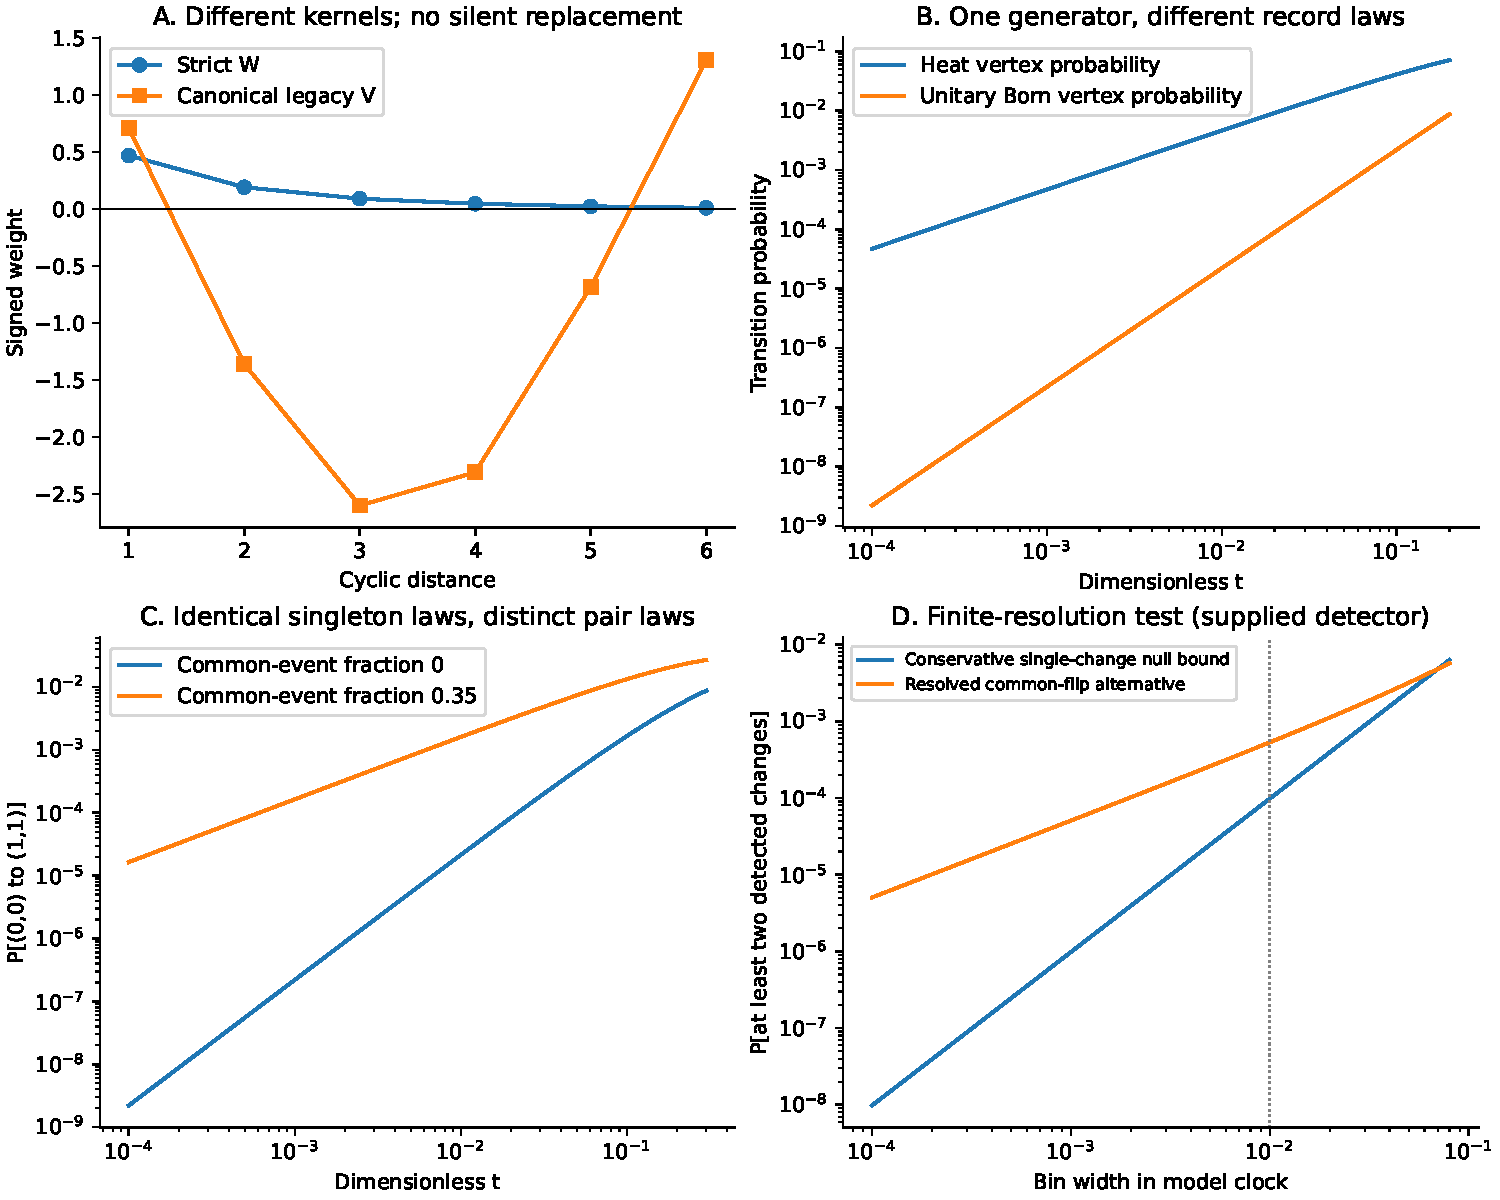
\includegraphics[width=\textwidth]{findings.pdf}}{}
The figure uses only the declared mathematical models. It shows neither
experimental data nor a simulation of the universe.

\section{The complete thirty-step adaptive chain}
\subsection*{01. ST8549 -- Can both raw kernels be Markov conductances?}
\noindent\textbf{Outcome.} Strict is positive; the declared raw Legacy* profile is signed and fails the rate test.\par
\noindent\textbf{Status.} Proven (conditional; see proof)\par
\noindent\textbf{Next-step rationale.} Instead of taking absolute values silently, retain signs in a doubled state space.\par\medskip
\subsection*{02. ST8550 -- Can legacy signs be retained in a positive stochastic cover?}
\noindent\textbf{Outcome.} A 24-state positive double cover has unsigned-even and signed-odd Laplacian sectors.\par
\noindent\textbf{Status.} Proven (conditional; see proof)\par
\noindent\textbf{Next-step rationale.} A shifted signed amplitude is not a probability: test whether a positive gauge removes the distinction.\par\medskip
\subsection*{03. ST8551 -- Can a diagonal sign or positive Doob gauge make raw legacy positive?}
\noindent\textbf{Outcome.} A negative triangle product obstructs sign switching to all-positive weights; positive diagonal similarity preserves each sign.\par
\noindent\textbf{Status.} Proven (conditional; see proof)\par
\noindent\textbf{Next-step rationale.} The sign degree of freedom must remain explicit; determine what a coarse observer loses.\par\medskip
\subsection*{04. ST8552 -- Does the sign-cover automatically complete legacy into strict?}
\noindent\textbf{Outcome.} Coarse mass is blind to every sign assignment, but its weights are |legacy|, not strict. The construction is not a completion map.\par
\noindent\textbf{Status.} Proven (conditional; see proof)\par
\noindent\textbf{Next-step rationale.} A mathematical dilation is insufficient: test the claimed dual dynamics at the level of vertex records.\par\medskip
\subsection*{05. ST8553 -- Are heat and unitary vertex records the same process?}
\noindent\textbf{Outcome.} Off-diagonal heat is t W\_ij+O(t\textasciicircum{}2); a finite Hamiltonian gives t\textasciicircum{}2 |H\_ij|\textasciicircum{}2+O(t\textasciicircum{}3). No positive linear clock identifies them.\par
\noindent\textbf{Status.} Proven (conditional; see proof)\par
\noindent\textbf{Next-step rationale.} Try an explicit repeated-measurement limit instead of Wick continuation.\par\medskip
\subsection*{06. ST8554 -- Does rapid projective measurement recover the strict heat operator?}
\noindent\textbf{Outcome.} With H scaled as delta\textasciicircum{}(-1/2), repeated vertex measurements converge to rates |H\_ij|\textasciicircum{}2. For H=A these are W\_ij\textasciicircum{}2, not W\_ij.\par
\noindent\textbf{Status.} Proven (conditional; see proof)\par
\noindent\textbf{Next-step rationale.} Try to compile the target rates explicitly, then test uniqueness of the compiled Hamiltonian.\par\medskip
\subsection*{07. ST8555 -- Can one compile strict heat from a Hamiltonian, uniquely?}
\noindent\textbf{Outcome.} Off-diagonal H\_ij=sqrt(W\_ij) exp(i theta\_ij) compiles W in that limit. Cycle phases and diagonals remain free and change coherent dynamics.\par
\noindent\textbf{Status.} Proven (conditional; see proof)\par
\noindent\textbf{Next-step rationale.} A compiled measurement limit introduces a Hamiltonian and instrument; test an exact quantum channel extension instead.\par\medskip
\subsection*{08. ST8556 -- Is there an exact completely positive heat embedding?}
\noindent\textbf{Outcome.} Rank-one jumps sqrt(W\_ij)|j\textgreater{}\textless{}i| give a trace-preserving Lindblad semigroup with exactly autonomous strict heat populations for all density matrices.\par
\noindent\textbf{Status.} Proven (conditional; see proof)\par
\noindent\textbf{Next-step rationale.} Exact embedding exists; test whether vertex records determine its coherence law.\par\medskip
\subsection*{09. ST8557 -- Do complete heat population records select a quantum completion?}
\noindent\textbf{Outcome.} Arbitrary nonnegative vertex dephasing changes coherences while preserving every autonomous population trajectory.\par
\noindent\textbf{Status.} Proven (conditional; see proof)\par
\noindent\textbf{Next-step rationale.} Test the desired original coherent generator H=A in the same extension.\par\medskip
\subsection*{10. ST8558 -- Can H=A be added without altering exact autonomous heat populations?}
\noindent\textbf{Outcome.} Not in the declared rank-one-jump plus vertex-dephasing class: autonomous heat for all density matrices forces H to be vertex-diagonal.\par
\noindent\textbf{Status.} Proven (conditional; see proof)\par
\noindent\textbf{Next-step rationale.} Do not identify two semigroups by a density-state Wick rotation; test normalization and linearity explicitly.\par\medskip
\subsection*{11. ST8559 -- Does normalized imaginary-time filtering define a universal physical channel?}
\noindent\textbf{Outcome.} It is nonlinear in the density matrix except for scalar filters. Unnormalized P rho P is a trace-decreasing CP operation, not deterministic heat on states.\par
\noindent\textbf{Status.} Proven (conditional; see proof)\par
\noindent\textbf{Next-step rationale.} Both stochastic and quantum lifts need extra premises. Test whether population consistency removes the stochastic freedom.\par\medskip
\subsection*{12. ST8560 -- Does exchangeability plus exact projective consistency force independent walkers?}
\noindent\textbf{Outcome.} No. Common vertex transpositions give a consistent exchangeable family with exactly the same single-particle generator Q and synchronized multi-particle jumps.\par
\noindent\textbf{Status.} Proven (conditional; see proof)\par
\noindent\textbf{Next-step rationale.} The fully synchronous law is reducible. Try irreducibility, detailed balance and the full equilibrium law as possible selectors.\par\medskip
\subsection*{13. ST8561 -- Do irreducibility, reversibility and a product-uniform equilibrium select the kinetics?}
\noindent\textbf{Outcome.} No. Every mixture 0\textless{}=theta\textless{}1 is irreducible and reversible with the identical product-uniform equilibrium and exact singleton heat.\par
\noindent\textbf{Status.} Proven (conditional; see proof)\par
\noindent\textbf{Next-step rationale.} Static Shannon entropy is therefore insufficient. Locate a dynamical observable separating these realizations.\par\medskip
\subsection*{14. ST8562 -- Which infinitesimal observation distinguishes the hidden common dynamics?}
\noindent\textbf{Outcome.} Pair coincidence / cross quadratic variation distinguishes the generators even when every single-particle trajectory and equilibrium law agrees.\par
\noindent\textbf{Status.} Proven (conditional; see proof)\par
\noindent\textbf{Next-step rationale.} Ask exactly which extra dynamical premise makes singleton rates determine the full generator.\par\medskip
\subsection*{15. ST8563 -- What minimal local premise yields a unique population generator?}
\noindent\textbf{Outcome.} Autonomous singleton generator Q at every configuration plus no simultaneous coordinate changes forces G\_N=sum\_k Q\textasciicircum{}(k). Exchangeability is unnecessary.\par
\noindent\textbf{Status.} Proven (conditional; see proof)\par
\noindent\textbf{Next-step rationale.} Replace the qualitative no-simultaneous-jump premise by a measurable, nonnegative witness.\par\medskip
\subsection*{16. ST8564 -- Can absence of common jumps be expressed without cancellation?}
\noindent\textbf{Outcome.} The pair budget B(x)=sum\_y g\_xy binom(K(x,y),2) is nonnegative and is zero exactly when every jump changes at most one coordinate.\par
\noindent\textbf{Status.} Proven (conditional; see proof)\par
\noindent\textbf{Next-step rationale.} A zero witness gives an exact theorem; derive a stable version for small nonzero coincidence rates.\par\medskip
\subsection*{17. ST8565 -- Does approximate pair locality bound the full finite-time model error?}
\noindent\textbf{Outcome.} With identical autonomous singleton rates, sup\_x B(x)\textless{}=epsilon implies sup\_x TV(P\_t(x,.),P\_ind,t(x,.))\textless{}=min(1,2 epsilon t).\par
\noindent\textbf{Status.} Proven (conditional; see proof)\par
\noindent\textbf{Next-step rationale.} Challenge the bound and its assumptions using many exchangeable particles with small jumps.\par\medskip
\subsection*{18. ST8566 -- Do exchangeability and a deterministic large-population limit select shot noise?}
\noindent\textbf{Outcome.} No. Uniformly chosen pairs with rate theta W/(N-1), mixed with single jumps, have the same mean heat and O(1/N) empirical variance but an altered noise prefactor.\par
\noindent\textbf{Status.} Proven (conditional; see proof)\par
\noindent\textbf{Next-step rationale.} This family is not projectively consistent across N. Test whether moment data can certify the missing event structure directly.\par\medskip
\subsection*{19. ST8567 -- Which raw-event inequalities survive arbitrary nonnegative jump rates?}
\noindent\textbf{Outcome.} Local integer-count cumulants obey kappa2\textgreater{}=|kappa1| and kappa4\textgreater{}=kappa2; equality in the latter excludes all marks with |k|\textgreater{}=2.\par
\noindent\textbf{Status.} Proven (conditional; see proof)\par
\noindent\textbf{Next-step rationale.} These are instantaneous raw-count statements. Attempt to falsify their use with ordinary detector binning.\par\medskip
\subsection*{20. ST8568 -- Can an ordinary detector make valid Poisson events appear to violate the local count bound?}
\noindent\textbf{Outcome.} Yes. A one-click-per-bin threshold maps Poisson arrivals to Bernoulli clicks, with variance/mean=exp(-lambda Delta)\textless{}1. Finite-bin data cannot be inserted into the instantaneous theorem.\par
\noindent\textbf{Status.} Proven (conditional; see proof)\par
\noindent\textbf{Next-step rationale.} Separate removable loss from irreversible thresholding and test whether a robust coincidence protocol exists.\par\medskip
\subsection*{21. ST8569 -- Which detector imperfection preserves the zero-coincidence theorem?}
\noindent\textbf{Outcome.} Independent resolution-preserving Bernoulli thinning gives B\_observed=eta\textasciicircum{}2 B. For eta\textgreater{}0 it preserves the exact zero set; a quantitative bound needs a lower efficiency bound.\par
\noindent\textbf{Status.} Proven (conditional; see proof)\par
\noindent\textbf{Next-step rationale.} Finite bins mix multiple events. Bound that contamination instead of assuming it vanishes.\par\medskip
\subsection*{22. ST8570 -- Can finite time resolution still test absence of simultaneous changes?}
\noindent\textbf{Outcome.} With a finite escape bound Lambda, a single-change null has Pr(at least two detected changes)\textless{}= (Lambda Delta)\textasciicircum{}2/2. A resolved joint event gives a positive order-Delta lower bound.\par
\noindent\textbf{Status.} Proven (conditional; see proof)\par
\noindent\textbf{Next-step rationale.} The rate orders separate analytically; compute a finite-sample test without synthetic-data fitting.\par\medskip
\subsection*{23. ST8571 -- Does the proposed rate-order test have a finite resource specification?}
\noindent\textbf{Outcome.} For independently reset trials a predeclared binomial upper-tail test controls the null and has high calculated power in the supplied two-particle model. No physical trial was performed.\par
\noindent\textbf{Status.} Proven conditional test rule; numerical tails supplemented by exact rational bounds\par
\noindent\textbf{Next-step rationale.} Attempt to destroy identifiability with an uncalibrated but nondegenerate detector.\par\medskip
\subsection*{24. ST8572 -- Can unknown event merging exactly hide common dynamics?}
\noindent\textbf{Outcome.} Yes. One-click-per-event reporting of the common-flip mixture and independently thinned single flips can produce the same entire nonzero Poisson record law despite different microscopic generators.\par
\noindent\textbf{Status.} Proven (conditional; see proof)\par
\noindent\textbf{Next-step rationale.} Even a mark-preserving detector may leave a clock/efficiency ambiguity. Test the full record likelihood, not just its mean.\par\medskip
\subsection*{25. ST8573 -- Does full resolved-count likelihood determine both clock and efficiency?}
\noindent\textbf{Outcome.} No. The two-particle count law has only c1,c2; a simultaneous change of w,theta,eta preserves both and hence every counting distribution.\par
\noindent\textbf{Status.} Proven (conditional; see proof)\par
\noindent\textbf{Next-step rationale.} Operational nonuniqueness is explicit. Audit the earlier nonlinear/prism and inverse-action alternatives before the final synthesis.\par\medskip
\subsection*{26. ST8574 -- Can the failed pure-parity kinetic counterexample be repaired honestly?}
\noindent\textbf{Outcome.} Adding an explicitly declared symmetric field gives two flip-energy magnitudes, so Metropolis and heat-bath cease to differ only by a clock. The original pure-parity proportionality is retained.\par
\noindent\textbf{Status.} Proven (conditional; see proof)\par
\noindent\textbf{Next-step rationale.} Equilibrium geometry fails to select kinetics. Test the analogous inverse-propagator-to-action claim.\par\medskip
\subsection*{27. ST8575 -- Does a supplied propagator determine the nonlinear variational theory?}
\noindent\textbf{Outcome.} No. Every S\_lambda=phi\textasciicircum{}T M phi/2-J\textasciicircum{}T phi+lambda sum phi\_i\textasciicircum{}4, lambda\textgreater{}=0, has the identical zero-source Hessian and linear response M\textasciicircum{}-1 but different cubic response.\par
\noindent\textbf{Status.} Proven (conditional; see proof)\par
\noindent\textbf{Next-step rationale.} Test whether hidden-state compression can select the missing dynamical response from the same static Green data.\par\medskip
\subsection*{28. ST8576 -- Does exact static Green/Schur compression select a hidden memory law?}
\noindent\textbf{Outcome.} No. Positive two-variable actions have identical coarse static Green function but different rational response and exponential memory; iteration does not remove the unsourced hidden parameters.\par
\noindent\textbf{Status.} Proven (conditional; see proof)\par
\noindent\textbf{Next-step rationale.} The surviving ambiguities occur in signs, quantum instruments, collective jumps, interactions and memory. Formulate only the no-go actually supported by explicit models.\par\medskip
\subsection*{29. ST8577 -- Can the audited finite FIN data logically determine a unique collective physical realization?}
\noindent\textbf{Outcome.} Not in the stated finite Markov completion class: same W, all singleton paths, product equilibrium, detailed balance, projective consistency and FIN graph symmetries coexist with different pair records.\par
\noindent\textbf{Status.} Proven (conditional; see proof)\par
\noindent\textbf{Next-step rationale.} This is not a universal impossibility of future physics. Close with a premise-removal and robustness audit of the smallest demonstrated positive bridge.\par\medskip
\subsection*{30. ST8578 -- Which rigorously narrowed bridge survives premise removal and perturbations?}
\noindent\textbf{Outcome.} In a declared finite CTMC, autonomous singleton Q plus zero pair-coincidence budget uniquely determines the generator; a small budget gives a stable TV bound. Initial law, clock, detector and the source of zero budget remain separate obligations.\par
\noindent\textbf{Status.} Proven (conditional; see proof)\par
\noindent\textbf{Next-step rationale.} Next: seek a strict-derived composition law forcing the nonnegative pair budget to vanish, or prove its independence in a precisely declared enlarged source class.\par\medskip


\end{document}
